\subsection{Model runs}
The model ran for 500 years for each of the 14 timesteps. Accounting for a total of 7000 years of model time. The timings are shown in \cref{table:masteps}. We see that the total integration time is quite long but in general manageable. We note that it would have been possible to significantly speed up our work by using many nodes in parallel instead of a single node in succession. This would be required for higher resolutions but was not attempted here.
As a metric for the stability of the model, we look at the globally averaged salinity and temperature change over time. This tells us the drift of the model. In \cref{table:mastepstable} we see the drift over the last 10 years of integration. We see that all of the models seem to have a drift of less than $10\mathrm{e}{-4}^{\circ}C$ per year and a salinity drift less than $10\mathrm{e}{-4} psu$ per year.

\begin{table}[H]
	\centering
	\begin{tabular}{lllll}
Year & $\Delta time$ & $time$ & $\Delta T$& $\Delta S$\\
present day & 1'01" & 8:30& -2.1978& -1.8629\\
5Ma& 1'01" & 8:30& -2.8292& -2.5038 \\
10Ma & 1'01" & 8:30& -2.7764& -1.8219\\
15Ma & 1'02" & 8:40& -6.1497& -2.6299\\
20Ma & 1'01" & 8:30&  -5.3202& -1.9109\\
25Ma & 1'02" & 8:40& -5.3201& -1.9341\\
30Ma & 1'03" & 8:30& -3.0994& -1.5755\\
35Ma & 1'00" & 8:30& -0.3163&-1.6289\\
40Ma & 1'02" & 8:40& -5.1253& -1.7728\\
45Ma & 1'00" & 8:20& -5.1196& -1.7066\\
50Ma & 1'00" & 8:20& -4.9925& -1.6592\\
55Ma & 1'01" & 8:30& -4.9158& -1.6586\\
60Ma & 1'02" & 8:40& -5.5853& -1.6902\\
65Ma & 1'03" & 8:50& -6.3302& -1.8980\\
	\end{tabular}

\caption{$\Delta time$ is the time per integration in minutes'seconds". $time$ is the time in hours:seconds for each run. $\Delta T$ is the average temperature gradient for the last 10 time steps in $10^{-4} C$ per year. $\Delta S$ is the average salinity gradient for the last 10 time steps in $10^{-4} psu$ per year.}
\label{table:mastepstable}
\end{table}


\subsection{Control setup}


To get an understanding of the quality of the model and thus if any of the results resemble reality, one can compare the present-day setup of the model to an existing model with realistic forcings. Also, the model can be compared to another similar higher resolution model. This can be a useful tool to see what aspects of the present-day situation are captured by the model and more importantly which nuances are lost. General circulation models with a resolution comparable to the model used in this paper often loose major features having to do with the overturning circulation (\cite{stone1990limitations}). Especially the restoring boundary conditions at the surface are troublesome where capturing artifacts of the thermohaline circulation is highly dependent on surface salinity and temperature profiles. This dependence is even further complicated by the highly idealized forcings used here (\cref{sec:forc_err}). To get a qualitative look at the error introduced in our model, the BSF and the MOC outputs are studied together with their temperature profiles. We compare our control setup with a run of our model with the original \cite{ECMWFForc} forcings scaled to 4-degrees. These are the same forcings used as a basis for making the idealized forcings as mentioned in \cref{sec:forcing_ideal}.
\begin{figure}[H]
	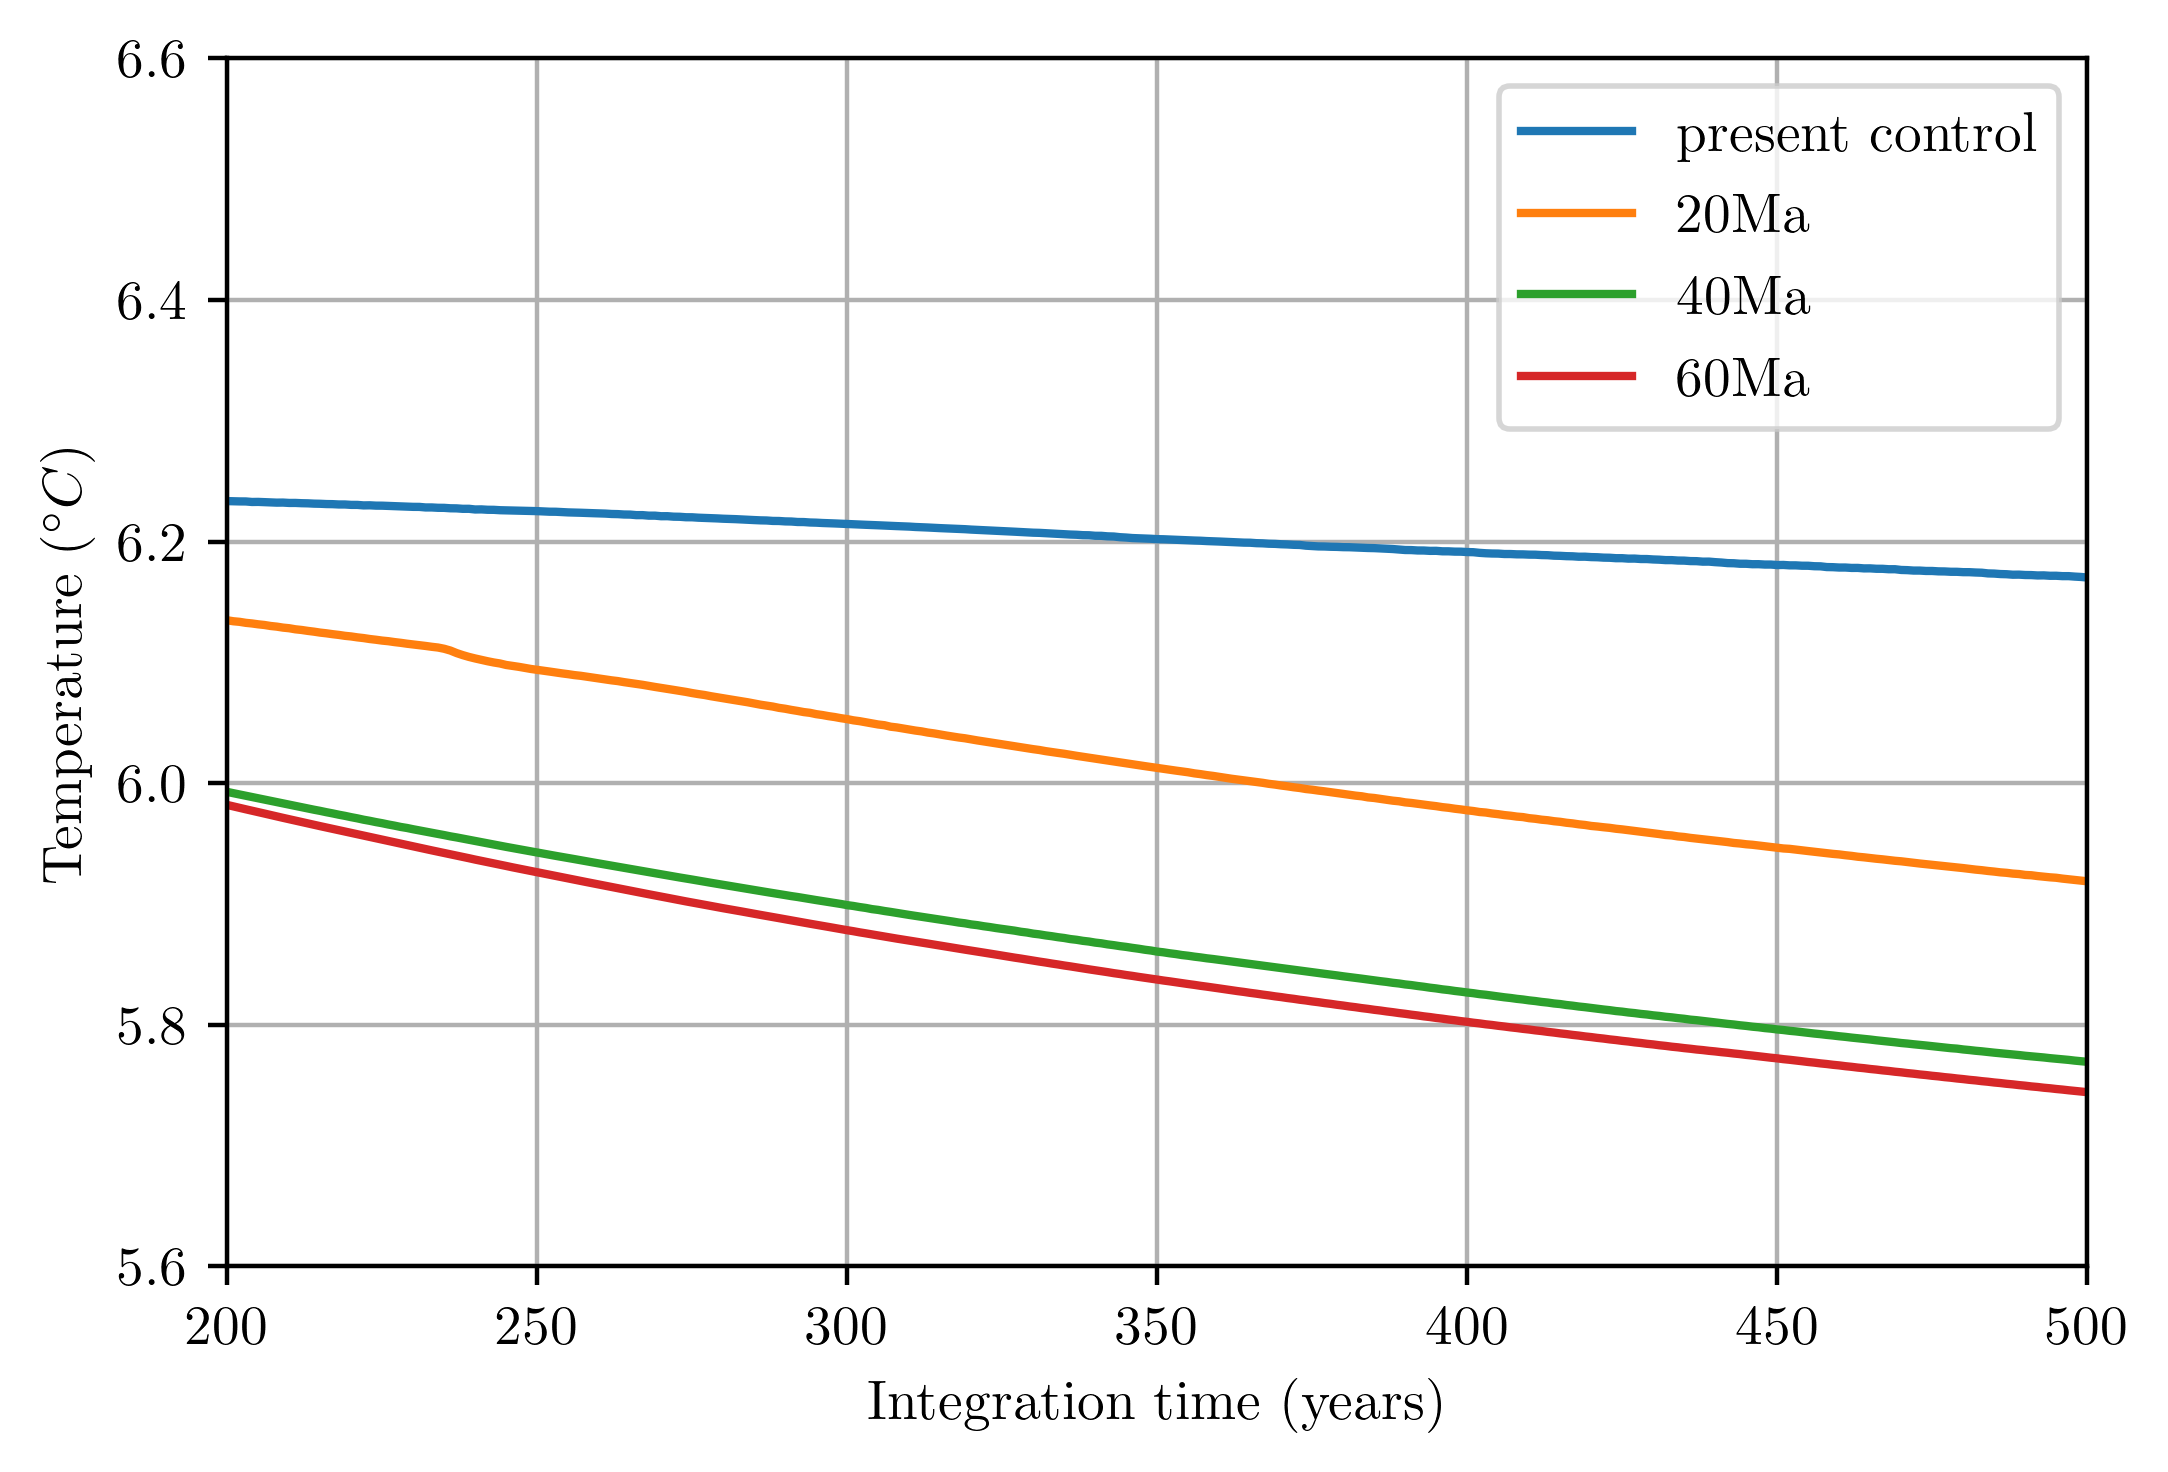
\includegraphics[width=\linewidth]{drift_integration.png}
	\caption{Total globally averaged temperature ($^{\circ}C$) for Present day (blue), 20Ma (orange), 40Ma (green) and 60Ma (red). From 200 to 500 years integration.}
	\label{fig:avtempgrph}
\end{figure}
\subsubsection{BSF control}
Too look at the quality of the barotropic stream function we compare the barotropic stream function with the control. In \cref{fig:bsf2_compared} we see the barotropic stream function compared. Here we see quite a few differences. Notably, the strength of the gyres is much weaker in our simplified forcings case. This can mostly be explained by the generally weaker wind stresses in these regions. Also, in our simplified model there is a notable absence of the sub polar gyre in the northern Atlantic. The difference in strength of the subtropical gyres is about $10Sv$ on average. Reaching a $20 Sv$ difference in the subtropical gyre in the Indian ocean. 


% Only showing a weaker subtropical gyre in the Indian ocean and a weaker gulf stream. In the temperature profile at 245 meters in depth there are however larger discrepancies. There is a $4^{\circ}C$ difference in temperature in the gulf stream and a $2^{\circ}C$ temperature difference in the Kuroshio gyre. This can be attributed to weaker SST forcing at the surface on these places because of the zonal mean nature of these forcings and also due to the shorter runlength of the model. Thus the model did not yet get addequate time to fully develop the flows (THIS COULD BE BETTER)


\end{multicols}
%example full width overturnings

\begin{figure}[H]

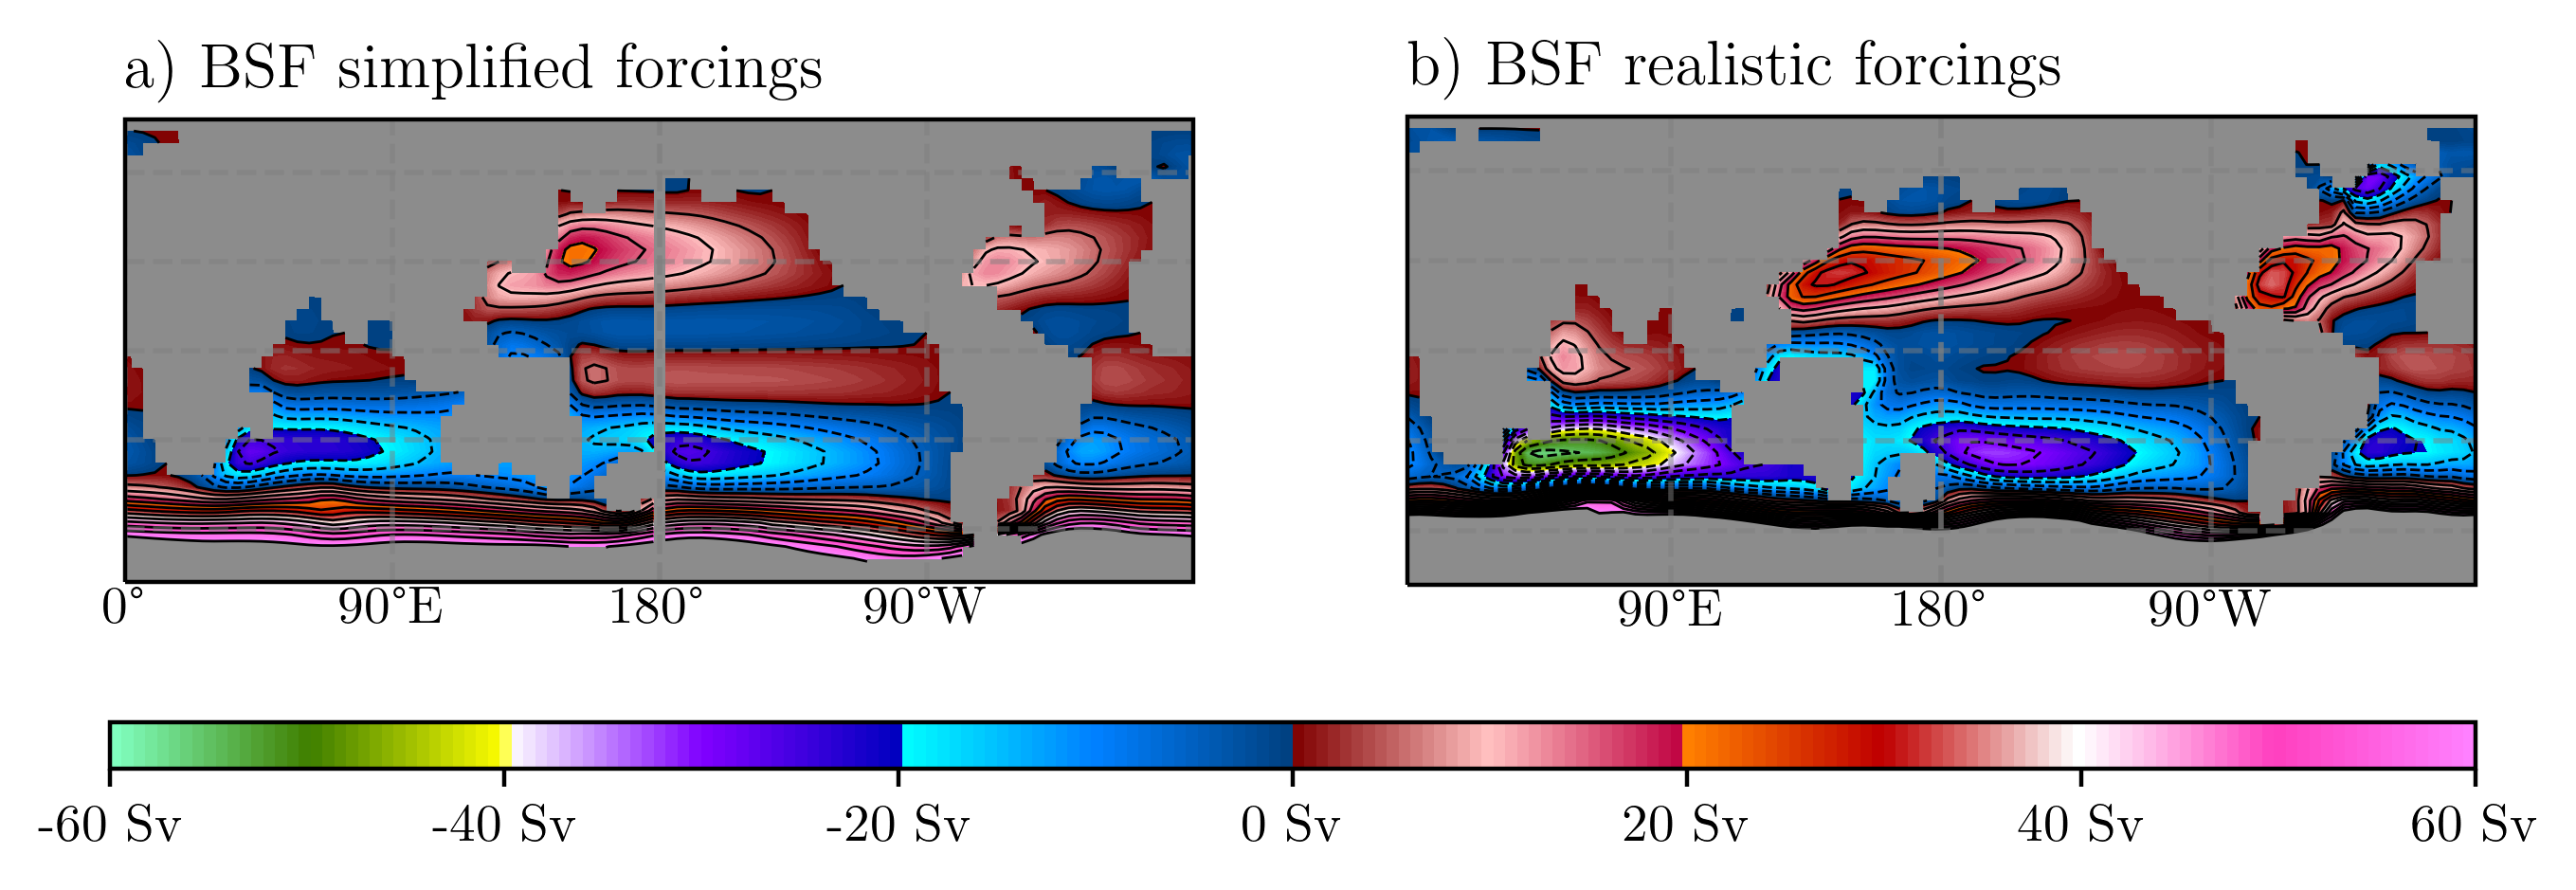
\includegraphics[width=\linewidth]{bsf_real_non.png}
\caption{Barotropic stream function with contours every 5 Sv. For \textbf{a)} simplified forcings and \textbf{b)} realistic forcings.}
\label{fig:bsf2_compared}
\end{figure}
\begin{figure}[H]
\begin{subfigure}{0pt}
	\caption*{}
	\label{fig:mocCompA}
\end{subfigure}
\begin{subfigure}{0pt}
	\caption*{}
	\label{fig:mocCompB}
\end{subfigure}
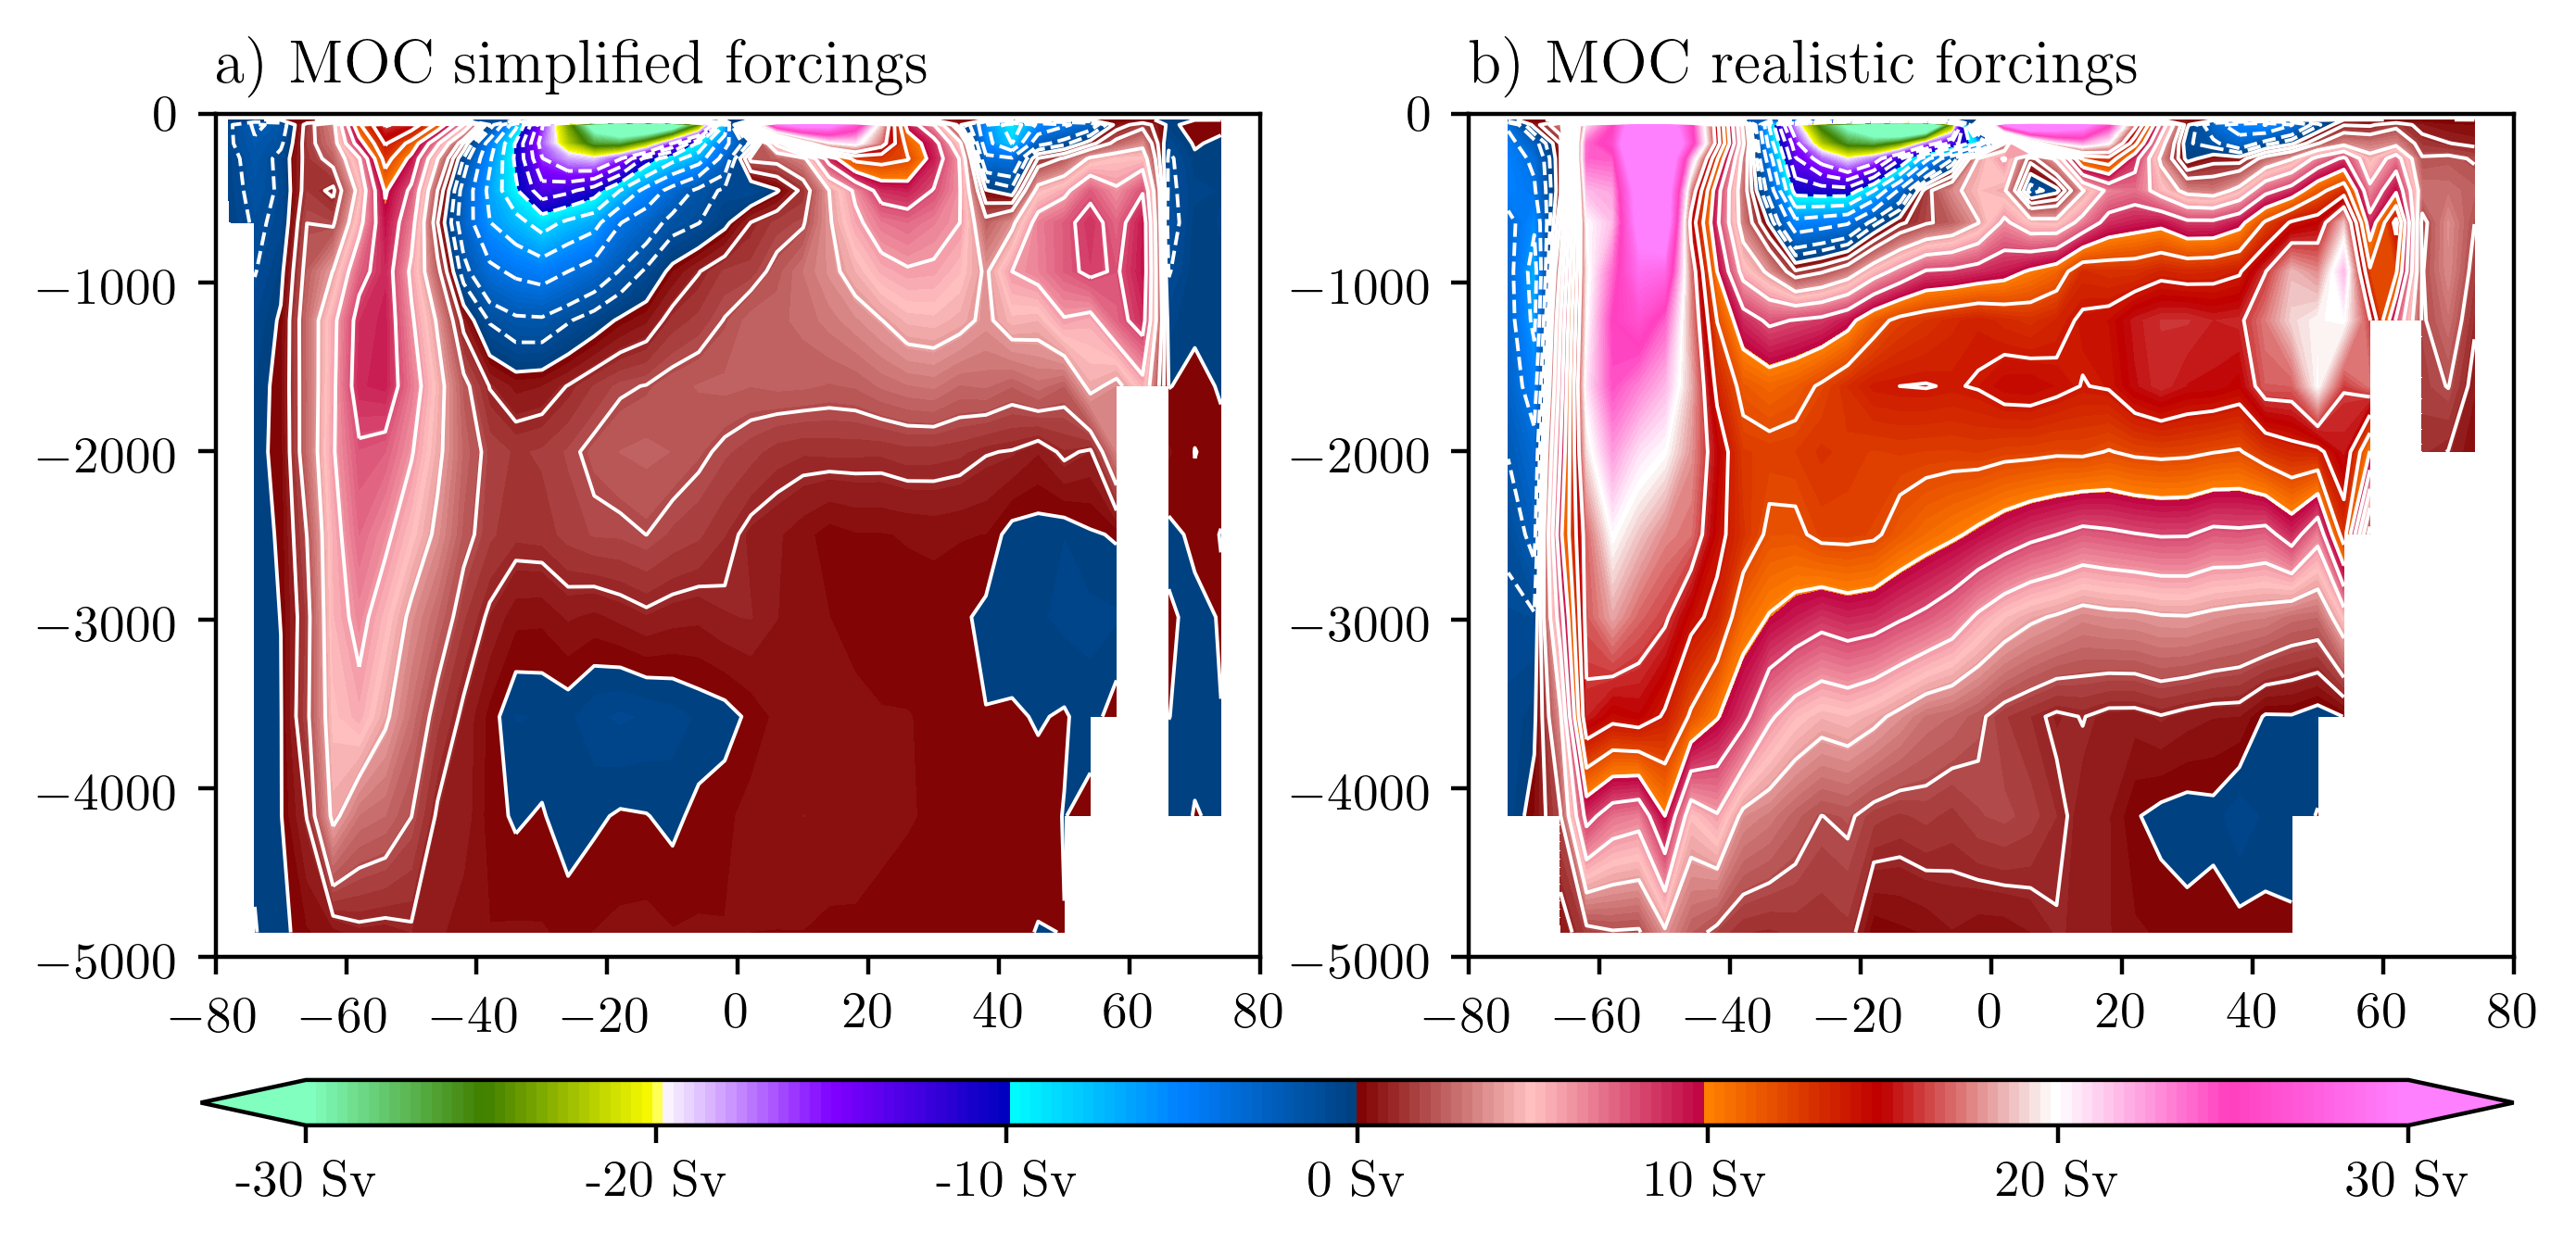
\includegraphics[width=\linewidth]{moc_forcings_real_fake.png}

\caption{MOC stream function with contours every 2 Sv. For \textbf{a)} simplified forcings and \textbf{b)} realistic forcings. Negative values (dashed lines) indicate counterclockwise circulation}
\label{fig:moc_compared}
\end{figure}

\begin{multicols}{2}

\subsubsection{Quality of the MOC} \label{sec:mocQual}
Next, we look at the MOC stream functions and compare them between the two models. Here we must note the difference in geometry between the two models. This is because we use an interpolated version in the simplified forcings case. That is different from the geometry used by Veros. In \cref{fig:moc_compared} we see the MOC stream function for the simplified and realistic models. Here the real problem of using simplified forcings is visible. The overturning circulation with the simplified forcings is extremely weak compared to the overturning circulation with simplified forcings. Compared to the model with realistic forcings in \cref{fig:mocCompB} we see that the NADW cell is much weaker in \cref{fig:mocCompA}. 

We note that several key features are not captured by both models. The first, most striking feature is the complete absence of the AABW cell. This is a common feature of low-resolution models used here. Furthermore it is noted that the absence of accurately simulated sea ice in both models contributes further to the quality of the southern ocean simulations. We also see a very large cell in the southern ocean around $60^{\circ} S$. This is a purely wind-driven cell not seen in the more realistic overturning from \cref{fig:moc_ex}. It is known as the "Deacon cell" (\cite{sverdrup1942oceans}; \cite{deacon1933general}).